\documentclass{article}
\usepackage{tikz}

% Componentes
\usepackage[utf8]{inputenc} % Codificación de entrada
\usepackage[T1]{fontenc} % Codificación de fuente

\usepackage{amsmath,amsfonts,amssymb} % Paquetes de matemáticas
\usepackage{graphicx} % Para insertar figuras
\usepackage{cite} % Para referencias
\usepackage{hyperref} % Para enlaces

% Título, autores, etc.
\title{Red neuronal 1}
\author{Jorge Butragueño Nieto}
\date{\today}

\begin{document}
	
	\maketitle
	
	\begin{abstract}
		Estudio de una red neuronal sencilla con tres nodos de entrada, dos capas ocultas de dos y cuatro nodos respectivamente, y finalmente un nodo en la capa de salida.
	\end{abstract}
	\section{Introducción}
	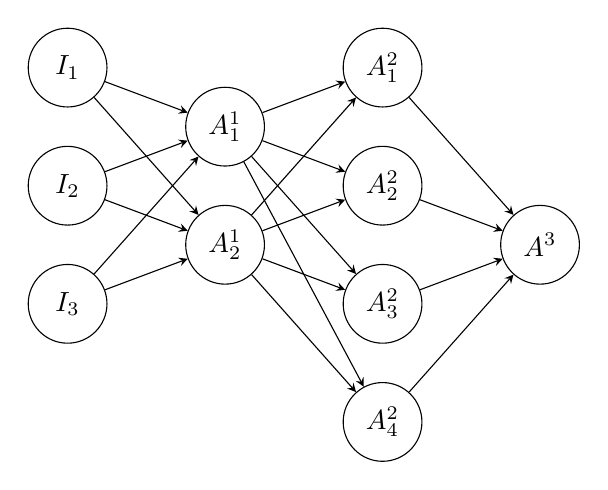
\begin{tikzpicture}[x=2cm, y=1.5cm, >=stealth]
		
		% Nodos de entrada
		\foreach \m/\l [count=\y] in {1,2,3}
		\node [circle, draw, minimum size=1cm] (input-\m) at (0,-\y) {$I_\m$};
		
		% Primera capa oculta
		\foreach \m [count=\y] in {1,2}
		\node [circle, draw, minimum size=1cm] (hidden1-\m) at (1,-\y-0.5) {$A^1_\m$};
		
		% Segunda capa oculta
		\foreach \m [count=\y] in {1,2,3,4}
		\node [circle, draw, minimum size=1cm] (hidden2-\m) at (2,-\y) {$A^2_\m$};
		
		% Nodo de salida
		\node [circle, draw, minimum size=1cm] (output) at (3,-2.5) {$A^3$};
		
		% Conexiones de la entrada a la primera capa oculta
		\foreach \i in {1,2,3}
		\foreach \j in {1,2}
		\draw [->] (input-\i) -- (hidden1-\j);
		
		% Conexiones de la primera capa oculta a la segunda capa oculta
		\foreach \i in {1,2}
		\foreach \j in {1,2,3,4}
		\draw [->] (hidden1-\i) -- (hidden2-\j);
		
		% Conexiones de la segunda capa oculta a la salida
		\foreach \i in {1,2,3,4}
		\draw [->] (hidden2-\i) -- (output);
		
	\end{tikzpicture}
	\\
	Queremos entrenar a la red para que dados tres valores binarios, devuelva 1 si hay más ceros que unos, y que devuelva 0 si es al contrario.
	Es decir:
	\[
	\text { [0, 0, 0] = 0, [0, 0, 1] = 0 }
	\hdots
	\text { [1, 1, 1] = 0}
	\]
	Podemos escribirlo en forma matricial, donde una fila
	\[
	X_{input} = \begin{bmatrix}
		1 & 0 & 0 \\
		0 & 1 & 0 \\
		0 & 0 & 1 \\
		0 & 0 & 0 \\
		0 & 1 & 1 \\
		1 & 0 & 1 \\
		1 & 1 & 0 \\
		1 & 1 & 1 \\
	\end{bmatrix}
	\text{  }
	y = \begin{bmatrix}
		0 \\ 0 \\ 0 \\ 0 \\ 1 \\ 1 \\ 1 \\ 1
	\end{bmatrix}
	\]

Recordemos que para que la red neuronal funcione hay que ajustar los pesos y las bias, los cuales almacenaremos de forma matricial.(En matrices nxm donde n: número de nodos de la capa previa, m: número de nodos de la capa actual)
	\[
	W_1  = \begin{bmatrix}
		w_{11} & w_{12}\\
		w_{21} & w_{22}\\
		w_{31} & w_{32} \\
		\end{bmatrix}
	W_2  = \begin{bmatrix}
		w_{11} & w_{12} & w_{13} & w_{14} & w_{15}\\
		w_{21} & w_{22} & w_{23} & w_{24} & w_{25}\\
	\end{bmatrix}
	W_3  = \begin{bmatrix}
	w_{11} \\ w_{21} \\ w_{31} \\ w_{41} \\ w_{51} \\
	\end{bmatrix}
	\]
	\[
	b1 = \begin{bmatrix}
		b_1 & b_2
	\end{bmatrix}
	b_2 = \begin{bmatrix}
		b_1 & b_2 & b_3 & b_4
	\end{bmatrix}
	b_3 = \begin{bmatrix}
		b_1
	\end{bmatrix}
	\]
	De esta forma podemos calcular Z de la siguiente manera:
	\[
	Z^1 = XW^1 + b^1
	\]

	Esto funciona ya que:
	\[
	Z^1 = \begin{bmatrix}
		x_{11} & x_{12} & x_{13} \\
		\vdots & \vdots & \vdots \\
		x_{81} & x_{82} & x_{83} \\
	\end{bmatrix}
	\begin{bmatrix}
		w_{11} & w_{12}\\
		w_{21} & w_{22}\\
		w_{31} & w_{32} \\
	\end{bmatrix}
	+
	\begin{bmatrix}
		b_1 & b_2
	\end{bmatrix}
	\]
	(Cabe decir que la bias al hacer la suma se expande para tener tantas filas como número de ejemplos, esto se ajusta automáticamente en bibliotecas como numpy.)
	Es decir 
	\[
	Z^1_{ij} = x_{i1} w_{1j} + x_{i2} w_{2j} + x_{i3} w_{3j} + b_j
	\text{     i=1,2,...,8. j=1,2.}
	\]
	\[
	A^1 = \sigma(Z^1)
	\]
	\[
	Z^2 = A^1 W^1 + b^1
	\]
	\[
	Z^2 = \begin{bmatrix}
		a_{11} & a_{12}\\
		\vdots & \vdots \\
		a_{81} & a_{82}
	\end{bmatrix}
	\begin{bmatrix}
		w_{11} & w_{12} & w_{13} & w_{14} & w_{15}\\
		w_{21} & w_{22} & w_{23} & w_{24} & w_{25}\\
	\end{bmatrix}
	+ 
	\begin{bmatrix}
		b_1 & b_2 & b_3 & b_4
	\end{bmatrix}	
	\]
	
	\[
	Z^2_{ij} = a_{i1}w_{1j} + a_{i2}w_{2j} + b_j \text{ i= 1,...,8. j = 1,2,3,4} 
	\]
	\[
	A^2 = \sigma(Z_2)
	\]
	
	\subsection{Error}
	El objetivo es encontrar los valores correctos de $w_1$, $w_2$, $b_1$ y $b_2$ para que el valor de la predicción coincida con el valor esperado. Para esto podemos considerar una función error $E(w_1, w_2, b_1, b_2)$ que depende de esos parámetros, ahora el objetivo será minimizarlo.
	\[
	E(\textbf{x}) = \frac{1}{2}(\hat{y} - y )^2
	\]
	Donde 
	\[
	\textbf{x} = \begin{bmatrix} 
		w_1\\
		b_1\\
		w_2\\
		b_2
	\end{bmatrix}
	\]
	$\hat{y}$ es la predicción dada por nuestro modelo.\\
	$y$ es el valor esperado.\\
	
	\section{Gradiente}
	Encontrar el mínimo se reduce a hallar calcular las derivadas, El gradiente de una función es la colección de todas las derivadas parciales:
	\[
	\mathbf{\nabla} f(\mathbf{x}) =
	\begin{bmatrix}
		\frac{\partial C(\mathbf{x})}{\partial w_1} \\
		\frac{\partial C(\mathbf{x})}{\partial b_1} \\
		\frac{\partial C(\mathbf{x})}{\partial w_2} \\
		\frac{\partial C(\mathbf{x})}{\partial b_2}
	\end{bmatrix}
	\]
	Sabemos que el gradiente apunta a la dirección de máximo crecimiento, es decir, si vamos en sentido contrario al gradiente estaremos ajustando los valores a un mínimo, justo lo que queremos
	Podemos hacer uso de la regla de la cadena para calcular las derivadas:
	\[
	\frac{\partial C}{\partial w_2} = \frac{\partial C}{\partial \hat{y}}\frac{\partial \hat{y}}{\partial w_2}
	\]
	\[
	\frac{\partial C}{\partial b_2} = \frac{\partial C}{\partial \hat{y}}\frac{\partial \hat{y}}{\partial b_2}
	\]
	Donde
	\[
	\frac{\partial C}{\partial \hat{y}} = \frac{\partial }{\partial \hat{y}} (\frac{1}{2}(\hat{y} - y )^2) = \hat{y} - y 
	\]
	\[
	\frac{\partial \hat{y}}{\partial w_2} = \frac{\partial}{\partial w_2} (w_2a_1 + b_2) = a_1
	\]
	\[
	\frac{\partial \hat{y}}{\partial w_2} = \frac{\partial}{\partial b_2} (w_2a_1 + b_2) = 1
	\]
	Es decir,
	\[
	\frac{\partial C}{\partial w_2} = (\hat{y} - y)a_1
	\]
	\[
	\frac{\partial C}{\partial w_2} = (\hat{y} - y)
	\]
	Para los primeros pesos podemos usar de la misma forma de la regla de la cadena
	\[
	\frac{\partial C}{\partial w_1} = \frac{\partial C}{\partial \hat{y}} \frac{\partial \hat{y}}{\partial a_1} \frac{\partial a_1}{\partial z_1} \frac{\partial z_1}{\partial w_1}
	\]
	\[
	\frac{\partial C}{\partial w_1} = \frac{\partial C}{\partial \hat{y}} \frac{\partial \hat{y}}{\partial a_1} \frac{\partial a_1}{\partial z_1} \frac{\partial z_1}{\partial b_1}
	\]
	faltaría por calcular:
	\[
	\frac{\partial \hat{y}}{\partial a_1} = \frac{\partial}{\partial a_1}(w_2a_1 + b_2) = w_2
	\]
	\[
	\frac{\partial a_1}{\partial z_1} =  \frac{\partial}{\partial z_1}(\text{ReLU}(z_1)) =
	\frac{\partial}{\partial z_1}
	\begin{cases}
		z_1, & \text{si } z_1 > 0 \\
		0, & \text{si } z_1 \leq 0
	\end{cases}
	=  
	\begin{cases}
		1, & \text{si } z_1 > 0 \\
		0, & \text{si } z_1 \leq 0
	\end{cases} 
	\]
	\[
	\frac{\partial z_1}{\partial w_1} = \frac{\partial}{\partial w_1} (w_1x_1 + b_1) = x_1
	\]
	\[
	\frac{\partial z_1}{\partial w_1} = \frac{\partial}{\partial b_1} (w_1x_1 + b_1) = 1
	\]
	Es decir:
	\[
	\frac{\partial C}{\partial w_1} = (\hat{y} - y)w_2\frac{\partial}{\partial z_1}(\text{ReLU}(z_1))x_1
	\]
	\[
	\frac{\partial C}{\partial b_1} = (\hat{y} - y)w_2\frac{\partial}{\partial z_1}(\text{ReLU}(z_1))
	\]
	De esta forma conocemos ya el gradiente:
	\[
	\nabla C = 
	\begin{bmatrix}
		(\hat{y} - y)a_1 \\
		(\hat{y} - y) \\
		(\hat{y} - y)w_2\frac{\partial}{\partial z_1}(\text{ReLU}(z_1))x_1 \\
		(\hat{y} - y)w_2\frac{\partial}{\partial z_1}(\text{ReLU}(z_1))
	\end{bmatrix}
	\]
	
	\section{Descenso por Gradiente}
	Ahora que conocemos el valor del gradiente en un punto \( \begin{bmatrix}
		w_1\\ 
		b_1\\
		w_2\\
		b_2
	\end{bmatrix}\) sólo tenemos que movernos en dirección opuesta al gradiente en un paso de tamaño \(\alpha\) 
	es decir 
	\[ \begin{bmatrix}
		w_1\\ 
		b_1\\
		w_2\\
		b_2
	\end{bmatrix} 
	\rightarrow
	\begin{bmatrix}
		w_1\\ 
		b_1\\
		w_2\\
		b_2
	\end{bmatrix} - \alpha \nabla C
	\]
	Con esto nos habríamos movido a un punto con un error un poco más pequeño que antes, y si repetimos este proceso, estaremos cada vez un poco más cerca, a este proceso de mejora continua se le denomina como entrenamiento. Y finalmente habrá conseguido unos valores que ajustan correctamente el resultado esperado.
	\newpage
	\section{Código}
	\begin{verbatim}
		import numpy as np
		
		# Función de activación ReLU
		def relu(x):
		return np.maximum(0, x)
		
		# Derivada de la función ReLU
		def relu_derivative(x):
		return np.where(x > 0, 1, 0)
		
		# Función de costo (error cuadrático medio)
		def mean_squared_error(prediction, target):
		return 0.5 * np.square(prediction - target)
		
		# Derivada de la función de costo respecto a la predicción
		def mse_derivative(prediction, target):
		return prediction - target
		
		# Pesos y sesgos iniciales
		w1 = 0.5  # Peso de la capa de entrada a la capa oculta
		b1 = 0.1  # Sesgo de la neurona en la capa oculta
		
		w_out = 0.4  # Peso de la capa oculta a la capa de salida
		b_out = 0.2  # Sesgo de la neurona en la capa de salida
		
		
		# Entrada (tamaño de la casa en metros cuadrados) y el precio objetivo (en miles de dólares)
		input_data = 50  # Tamaño de la casa
		target = 300  # Precio de la casa
		
		# Propagación hacia adelante
		z1 = w1 * input_data + b1  # Entrada a la neurona de la capa oculta
		a1 = relu(z1)  # Salida de la neurona de la capa oculta
		
		z_out = w_out * a1 + b_out  # Entrada a la neurona de salida
		prediction = z_out  # Como no aplicamos una función de activación en la salida, la predicción es z_out
		
		print(f"Predicción inicial: {prediction}")
		
		# Cálculo del error
		error = mean_squared_error(prediction, target)
		print(f"Error inicial: {error}")
		
		# Tasa de aprendizaje
		learning_rate = 0.00001
		
		# Derivada del error con respecto a la salida de la red (z_out)
		d_error_d_z_out = mse_derivative(prediction, target)
		
		# Derivada de z_out respecto a los pesos y sesgos en la salida
		d_z_out_d_w_out = a1
		d_z_out_d_b_out = 1
		
		# Actualización de pesos y sesgos de la capa de salida
		w_out -= learning_rate * d_error_d_z_out * d_z_out_d_w_out
		b_out -= learning_rate * d_error_d_z_out * d_z_out_d_b_out
		
		# Derivada de z_out respecto a la salida de la capa oculta (a1)
		d_z_out_d_a1 = w_out
		
		# Derivada del error respecto a la salida de la capa oculta (a1)
		d_error_d_a1 = d_error_d_z_out * d_z_out_d_a1
		
		# Derivada de la salida de la capa oculta (a1) respecto a su entrada (z1)
		d_a1_d_z1 = relu_derivative(z1)
		
		# Derivada de z1 respecto a los pesos y sesgos en la capa oculta
		d_z1_d_w1 = input_data
		d_z1_d_b1 = 1
		
		# Actualización de pesos y sesgos de la capa oculta
		w1 -= learning_rate * d_error_d_a1 * d_a1_d_z1 * d_z1_d_w1
		b1 -= learning_rate * d_error_d_a1 * d_a1_d_z1 * d_z1_d_b1
		
		print(f"Peso w1 actualizado: {w1}")
		print(f"Sesgo b1 actualizado: {b1}")
		print(f"Peso w_out actualizado: {w_out}")
		print(f"Sesgo b_out actualizado: {b_out}")
		
		# Número de iteraciones de entrenamiento
		epochs = 1000
		
		for epoch in range(epochs):
		# Propagación hacia adelante
		z1 = w1 * input_data + b1
		a1 = relu(z1)
		
		z_out = w_out * a1 + b_out
		prediction = z_out
		
		# Cálculo del error
		error = mean_squared_error(prediction, target)
		
		# Retropropagación
		d_error_d_z_out = mse_derivative(prediction, target)
		
		# Actualización de la capa de salida
		w_out -= learning_rate * d_error_d_z_out * d_z_out_d_w_out
		b_out -= learning_rate * d_error_d_z_out * d_z_out_d_b_out
		
		d_z_out_d_a1 = w_out
		d_error_d_a1 = d_error_d_z_out * d_z_out_d_a1
		d_a1_d_z1 = relu_derivative(z1)
		
		# Actualización de la capa oculta
		w1 -= learning_rate * d_error_d_a1 * d_a1_d_z1 * d_z1_d_w1
		b1 -= learning_rate * d_error_d_a1 * d_a1_d_z1 * d_z1_d_b1
		
		# Imprimir el progreso cada 100 iteraciones
		if epoch % 100 == 0:
		print(f"Iteración {epoch+1}/{epochs}, Error: {error}, Predicción: {prediction}")
		
		# Predicción final
		print(f"Predicción final después del entrenamiento: {prediction}")
		
	\end{verbatim}
	
	Muchas gracias por ver el vídeo $:)$
	
\end{document}
